\Exhibit{AkvelonRsSalary}{%
    Response from Revenue Service of Georgia showing \mrls salary before taxes, with a way to verify online\WithTr%
}

This statement from the Revenue Service of Georgia shows the total gross salary
received by \mrl as 167014.90 Georgian Lari.

This statement contains a QR code that opens this same document on the website
of the Revenue Service thus providing a way to verify its authenticity.

\begin{center}
    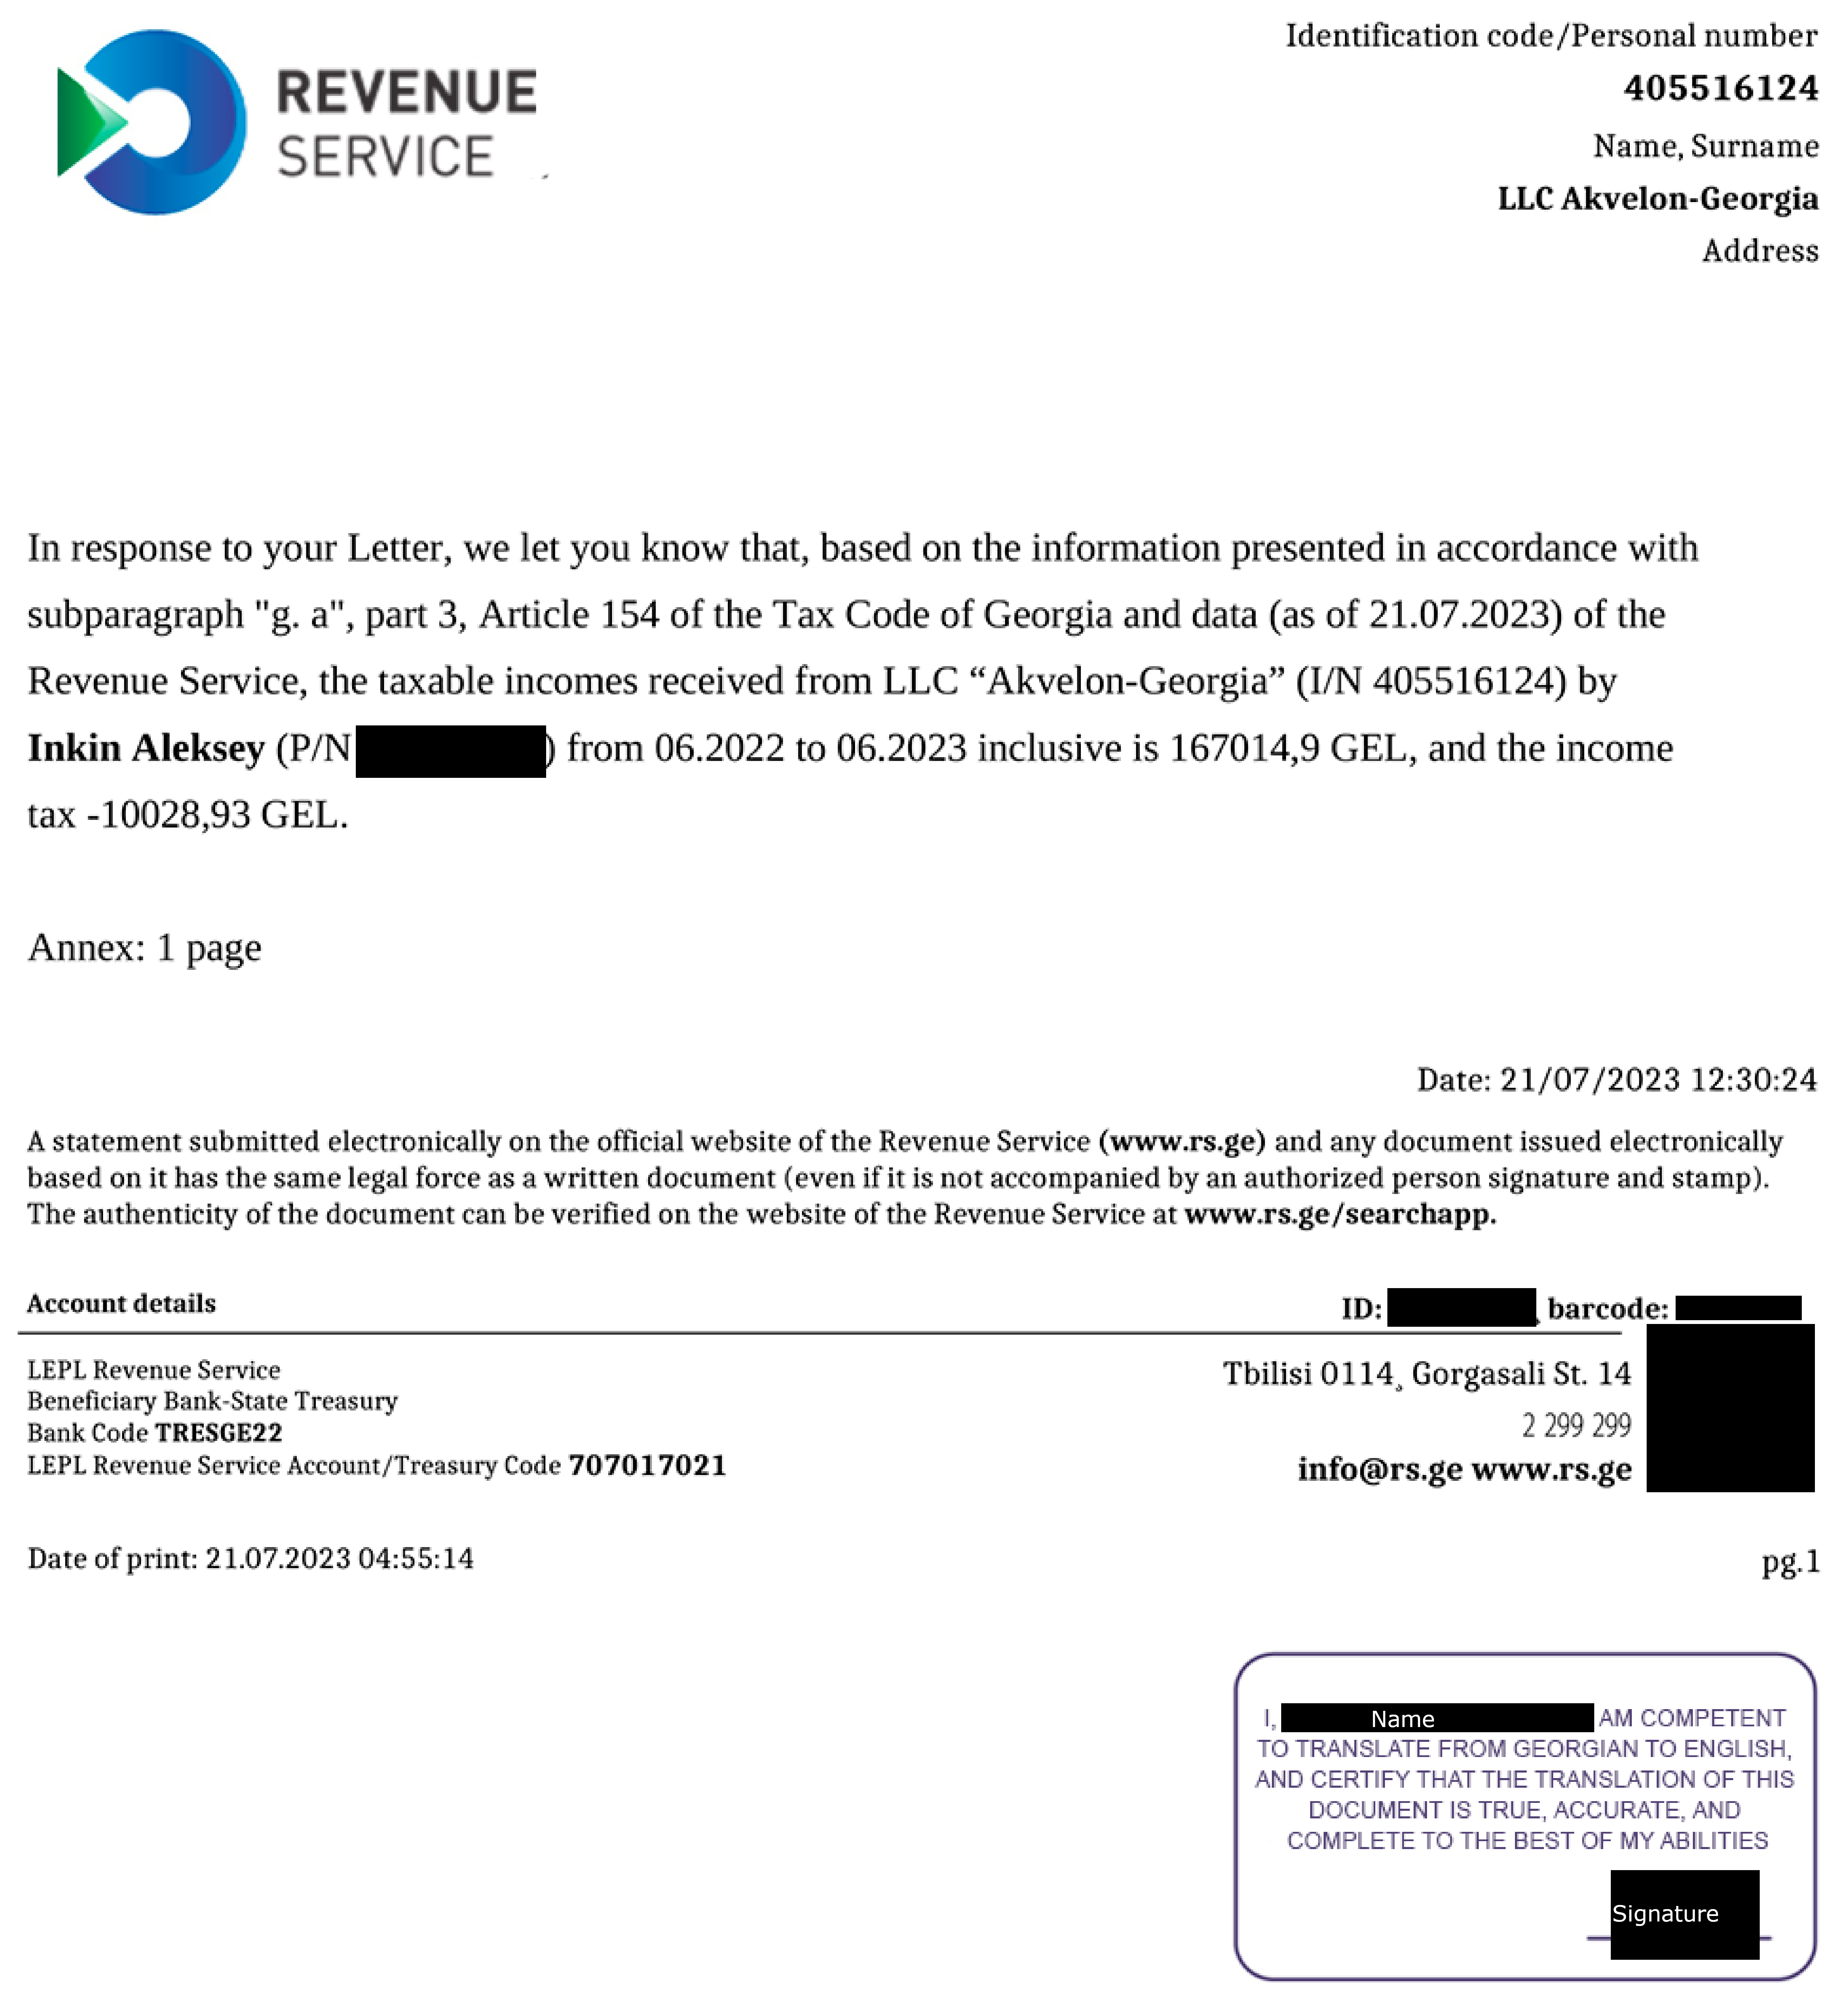
\includegraphics[width=35em]{rs-1_en_public}
\end{center}

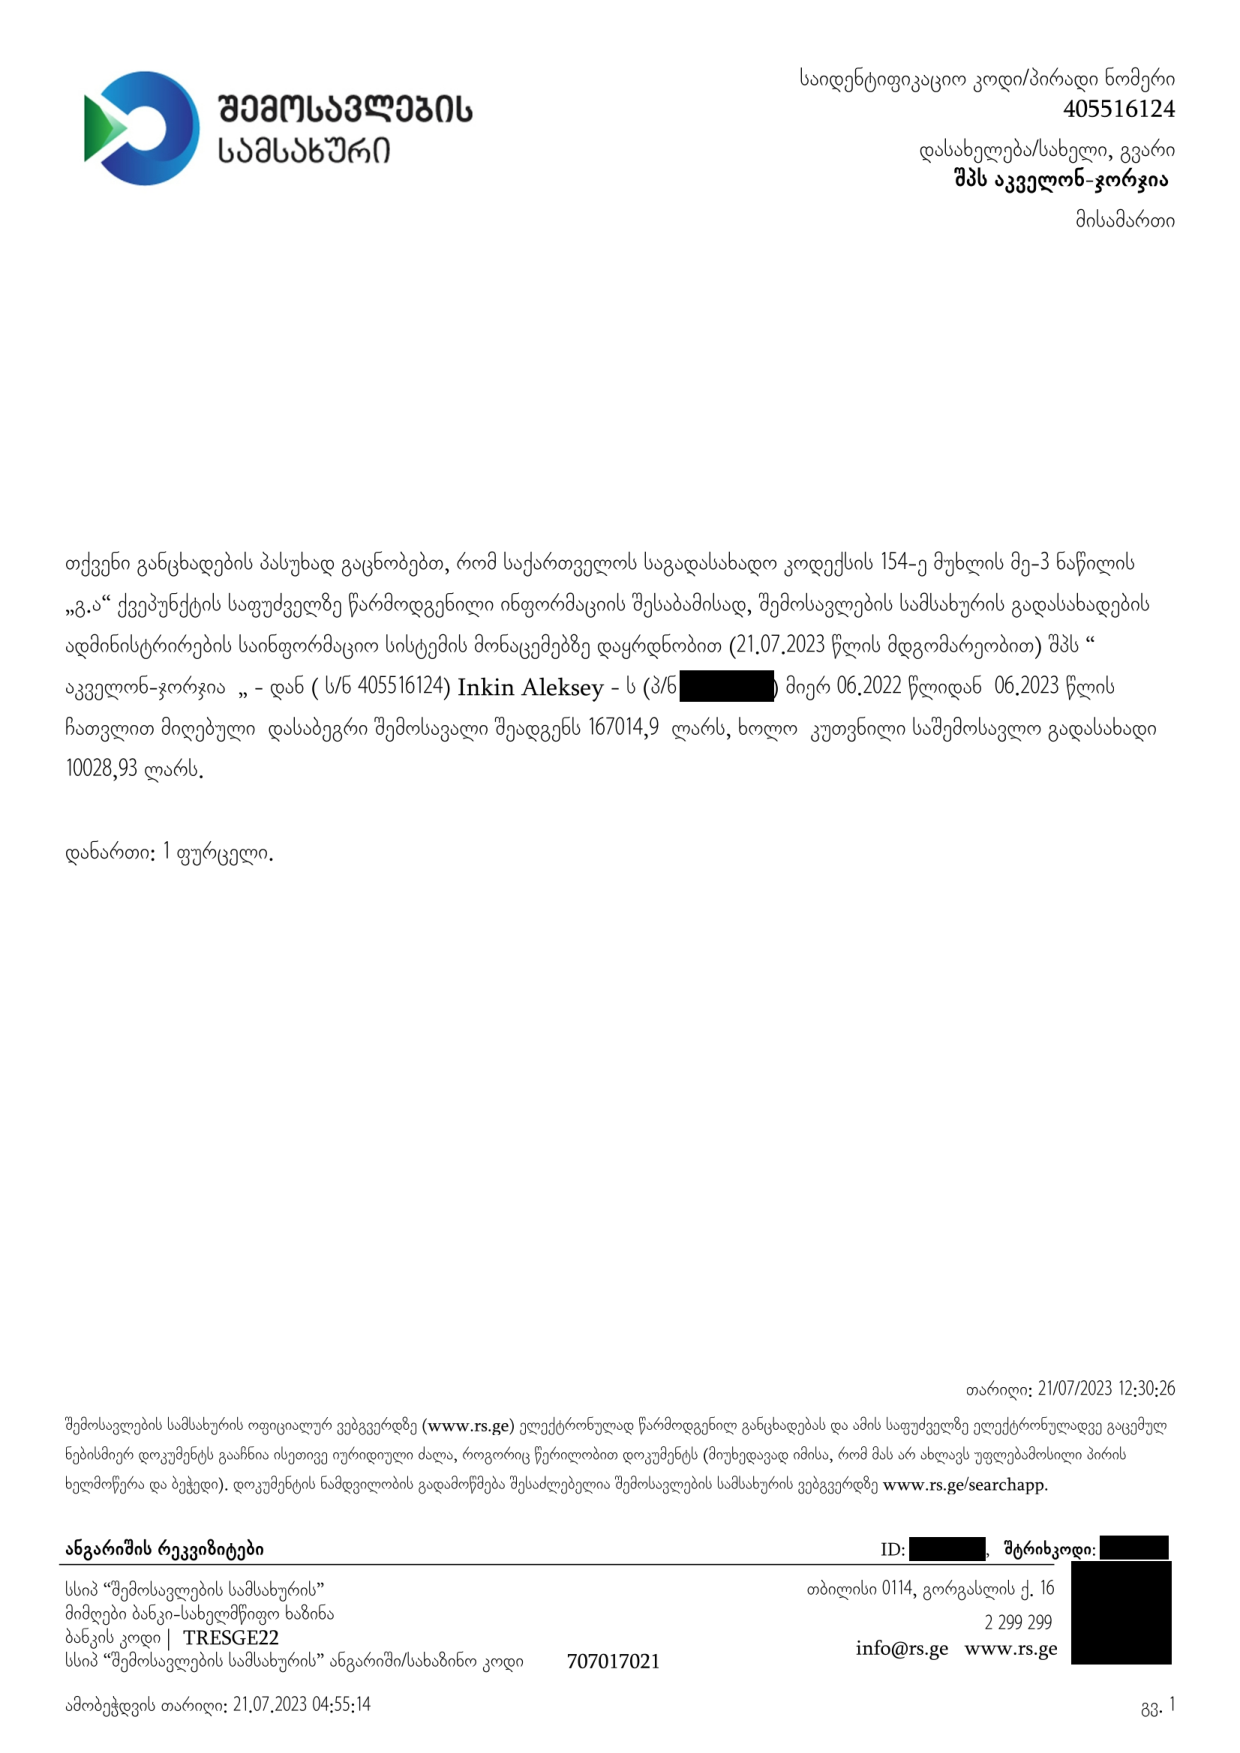
\includepdf[pages=-]{rs-1_public}

\begin{center}
    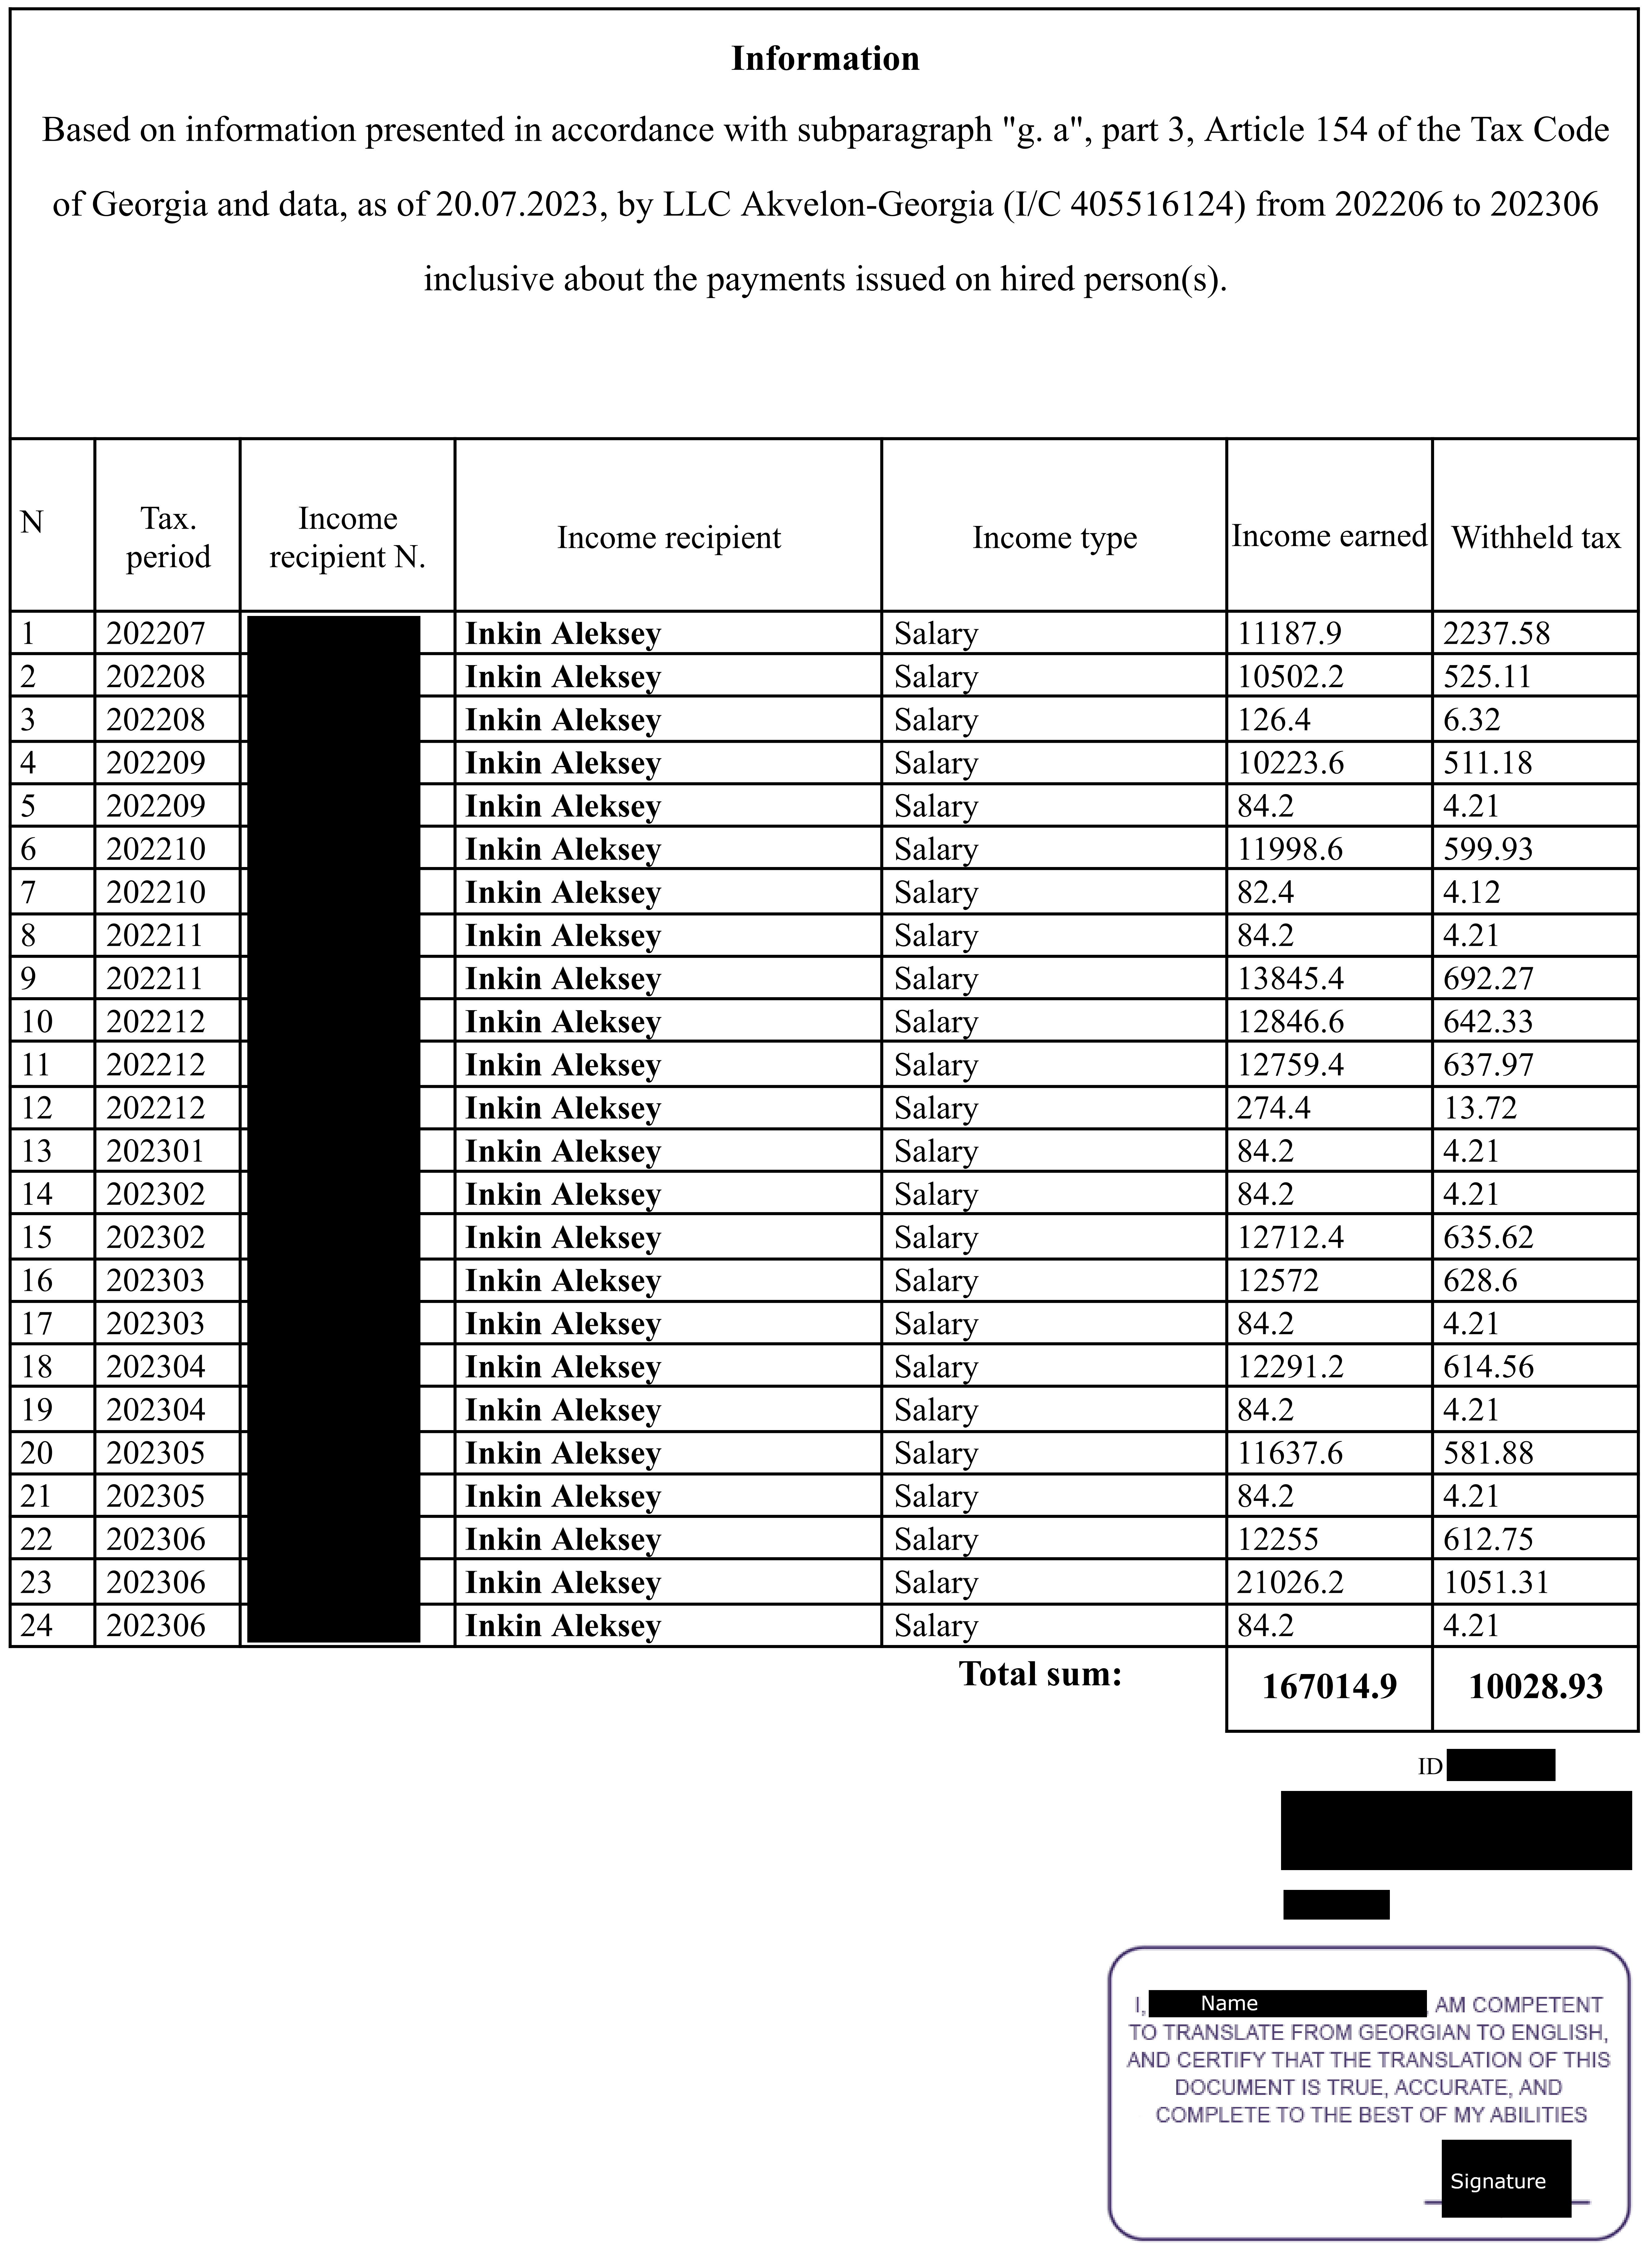
\includegraphics[width=35em]{rs-2_en_public}
\end{center}

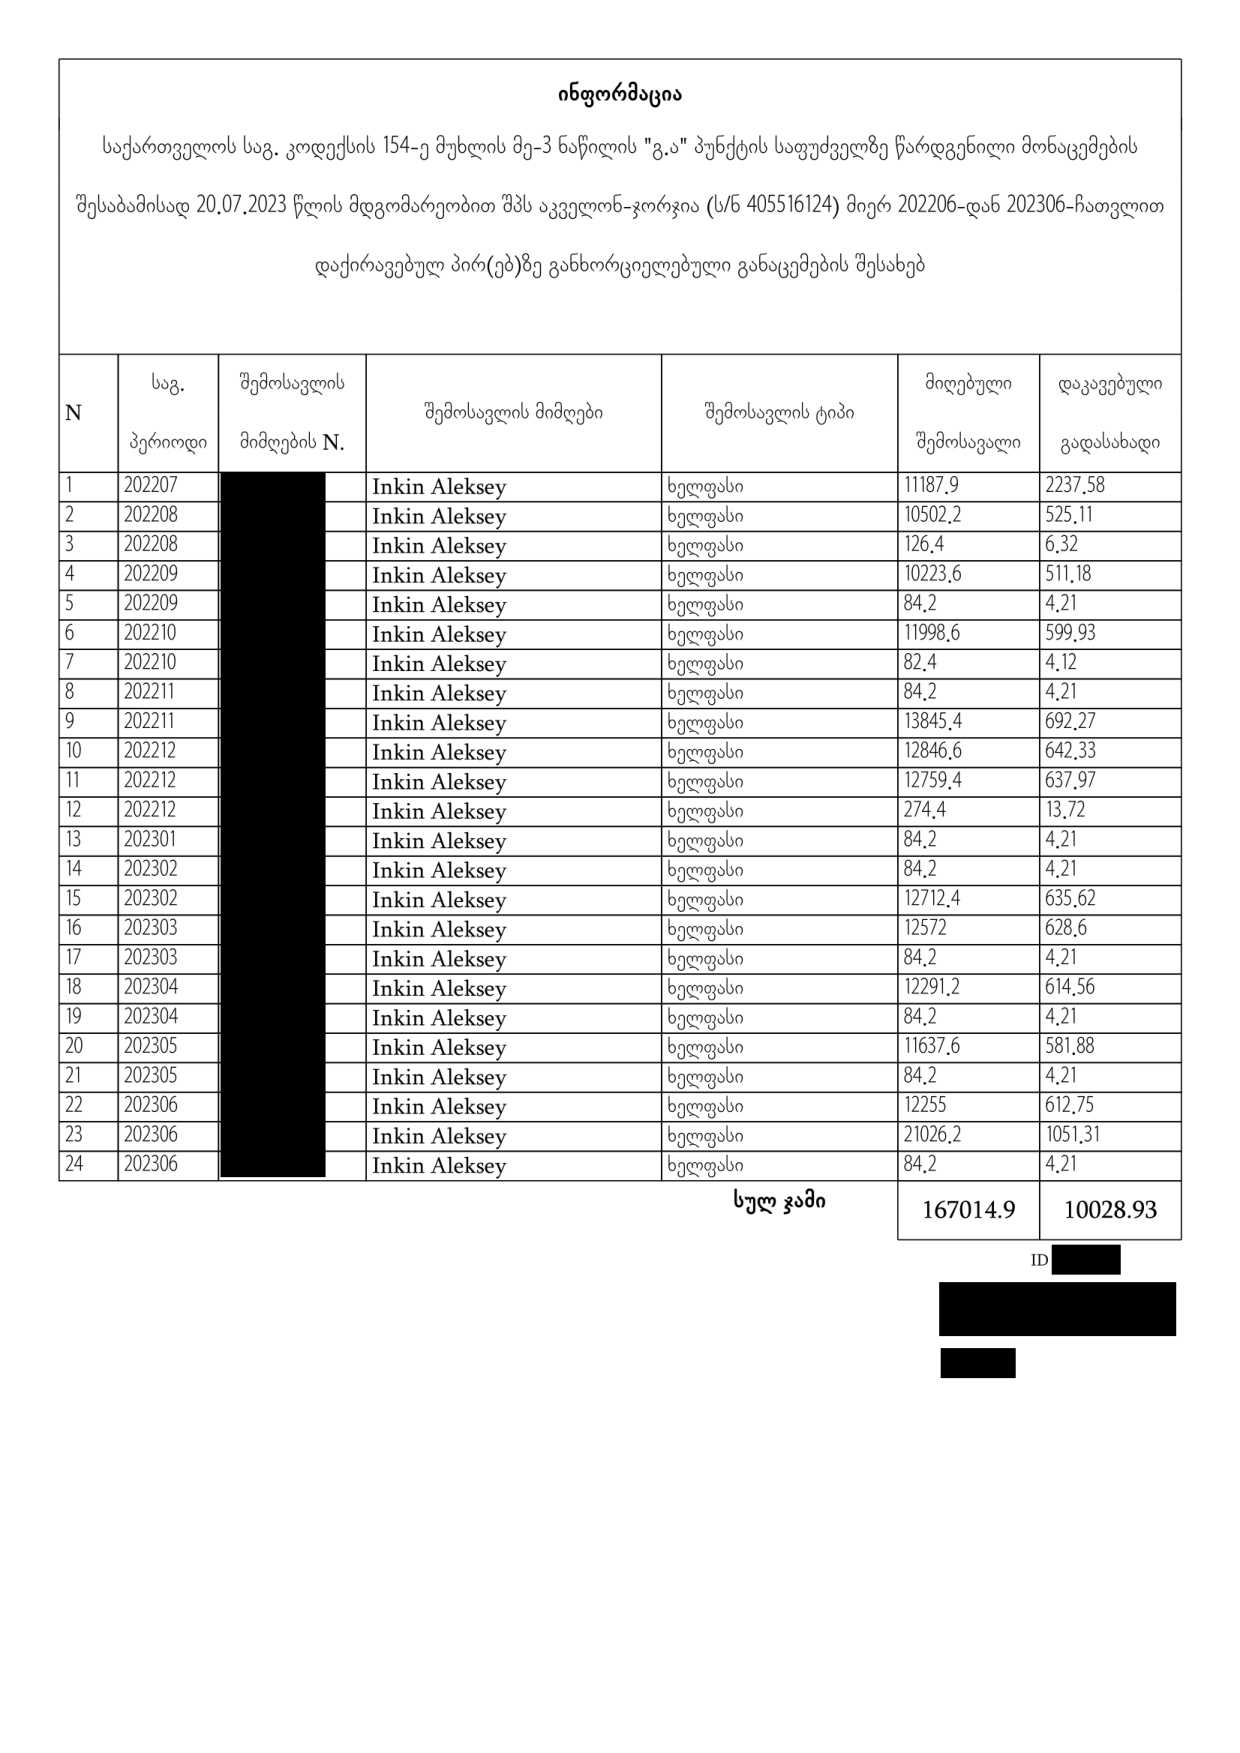
\includepdf[pages=-]{rs-2_public}

Alternatively, this online version can be reached at this address:
https://www.rs.ge/searchapp

The page that opens prompts for the Application ID (the 1st field)
and the Barcode number (the 2nd field).
Enter the following information as the document itself indicates:

\begin{tabular}{ll}
    Application ID: & <\dots> \\
    Barcode number: & <\dots> \\
\end{tabular}


In the popup window that opens, the two buttons open the two pages of the Revenue Service statement.

\begin{center}
    \includegraphics[width=35em]{rs-verification_en_public}
\end{center}

\begin{center}
    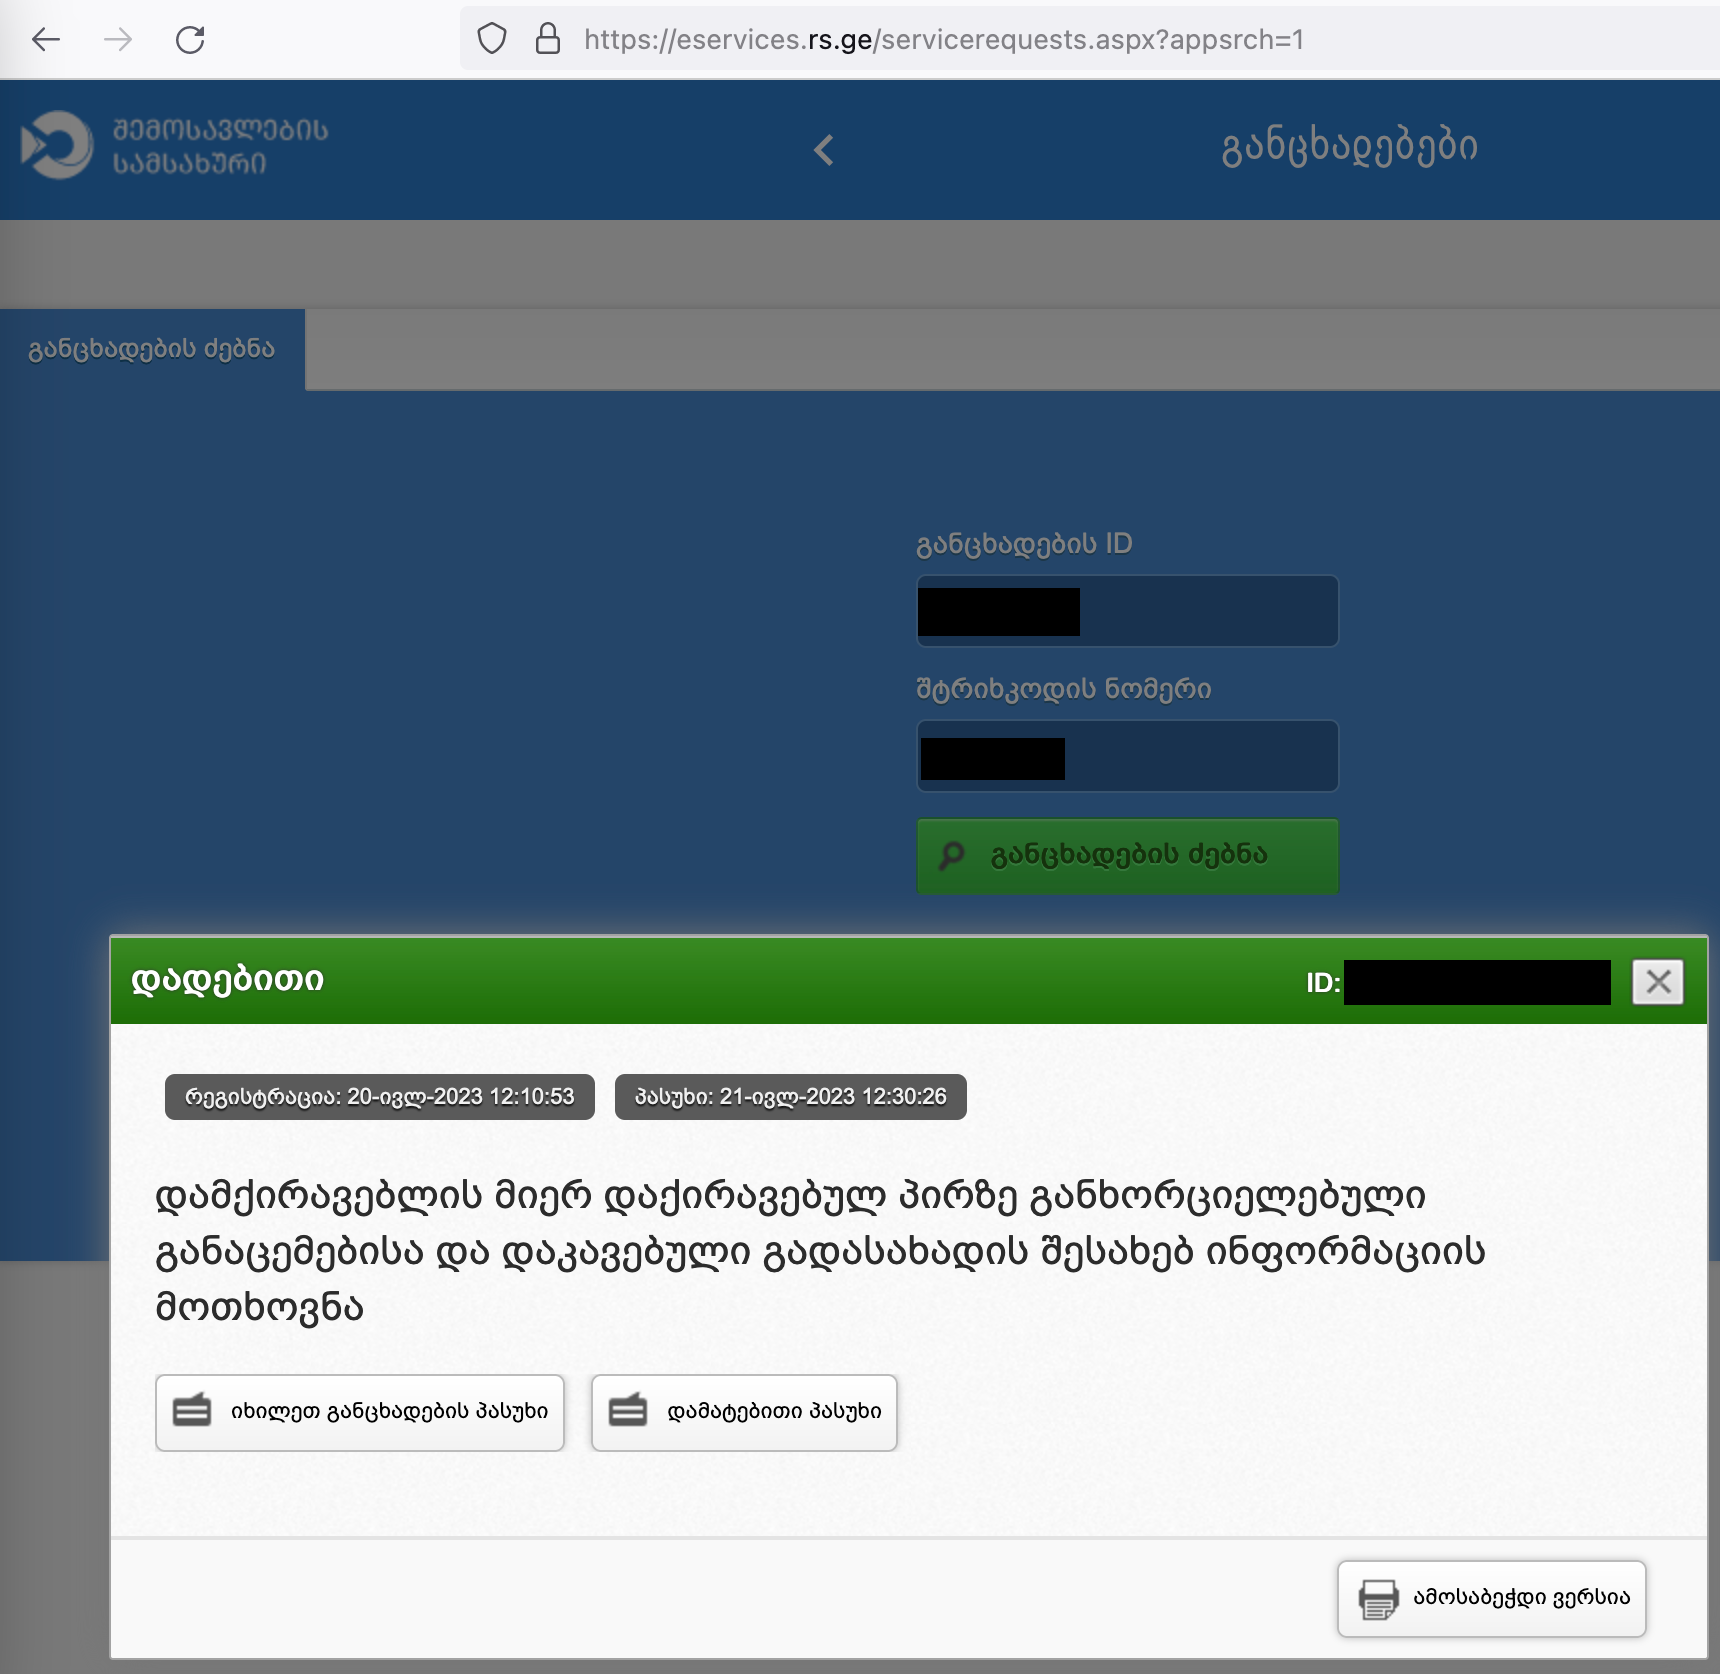
\includegraphics[width=35em]{rs-verification_public}
\end{center}

\pagebreak
